% arara: xelatex
%% arara: xelatex


% https://koalatea.io/r-knn-regression/
% http://freerangestats.info/blog/2017/04/09/propensity-v-regression
% https://economics.stackexchange.com/questions/45335/what-is-the-difference-between-ate-and-att
% https://kosukeimai.github.io/MatchIt/articles/matching-methods.html


\documentclass[14pt,xcolor=dvipsnames]{beamer}


% !TEX root = om_metrics_14.tex

%\usepackage{epsdice} % dice 1-6 for probability :)

% \usepackage[absolute,overlay]{textpos}

% \usefonttheme[onlymath]{serif}

\usefonttheme{professionalfonts}
% by default beamer changes math fonts for better visibility for projection
% this professionalfonst theme removes this behavior


\usepackage[orientation=portrait,size=custom,width=25.4,height=19.05]{beamerposter}




%25,4 см 19,05 см размеры слайда в powerpoint

\usetheme{metropolis}
\metroset{
  %progressbar=none,
  numbering=none,
  subsectionpage=progressbar,
  block=fill
}

%\usecolortheme{seahorse}

\usepackage{fontspec}
\usepackage{polyglossia}
\setmainlanguage{russian}


% \usepackage{fontawesome5} % removed [fixed]
\setmainfont[Ligatures=TeX]{Myriad Pro}
% \setsansfont{Myriad Pro}




% why do we need \newfontfamily:
% http://tex.stackexchange.com/questions/91507/
\newfontfamily{\cyrillicfonttt}{Myriad Pro}
\newfontfamily{\cyrillicfont}{Myriad Pro}
%\newfontfamily{\cyrillicfontbs}{Myriad Pro}
\newfontfamily{\cyrillicfontsf}{Myriad Pro}


% https://tex.stackexchange.com/questions/175860/why-does-unicode-math-break-the-kerning-of-accents-in-combination-with-amssymb
% "You shouldn't be using amssymb together with unicode-math"
\usepackage{amsmath}
\usepackage{amsthm} % amssymb 


% https://tex.stackexchange.com/questions/483722/
% \usepackage[MnSymbol]{mathspec}  % Includes amsmath.
% \usepackage{mathspec}  % Includes amsmath.
% \setmathsfont(Digits,Latin,Greek,Symbols)[Numbers={Lining,Proportional}]{Latin Modern Math}
% mathspec must be loaded earlier than amsmath



%\usepackage{bm}

% \usepackage{fdsymbol} % \nperp

% \usepackage{unicode-math} % \symbf
% \setmathfont{Latin Modern Math}



\usepackage{centernot}

\usepackage{graphicx}

\usepackage{wrapfig}
% \usepackage{animate} % animations :)
% \usepackage{tikz}
%\usetikzlibrary{shapes.geometric,patterns,positioning,matrix,calc,arrows,shapes,fit,decorations,decorations.pathmorphing}
% \usepackage{pifont}
\usepackage{comment}
\usepackage[font=small,labelfont=bf]{caption}
\captionsetup[figure]{labelformat=empty}
% \includecomment{techno}



%Расположение

\setbeamersize{text margin left=15 mm,text margin right=5mm} 
\setlength{\leftmargini}{38 pt}

%\usepackage{showframe}
%\usepackage{enumitem}
% \setlist{leftmargin=5.5mm}


%Цвета от дирекции

\definecolor{dirblack}{RGB}{58, 58, 58}
\definecolor{dirwhite}{RGB}{245, 245, 245}
\definecolor{dirred}{RGB}{149, 55, 53}
\definecolor{dirblue}{RGB}{0, 90, 171}
\definecolor{dirorange}{RGB}{235, 143, 76}
\definecolor{dirlightblue}{RGB}{75, 172, 198}
\definecolor{dirgreen}{RGB}{155, 187, 89}
\definecolor{dircomment}{RGB}{128, 100, 162}

\setbeamercolor{title separator}{bg=dirlightblue!50, fg=dirblue}

%Цвета блоков

% Голубой блок!
\setbeamercolor{block title}{bg=dirblue!30,fg=dirblack}
\setbeamercolor{block title example}{bg=dirlightblue!50,fg=dirblack}
\setbeamercolor{block body example}{bg=dirlightblue!20,fg=dirblack}

\AtBeginEnvironment{exampleblock}{\setbeamercolor{itemize item}{fg=dirblack}}
%\setbeamertemplate{blocks}[rounded][shadow]

% Набор команд для удобства верстки

% Набор команд для структуризации

%\newcommand{\quest}{\faQuestionCircleO}
%\faPencilSquareO \faPuzzlePiece \faQuestionCircleO  \faIcon*[regular]{file} {\textcolor{dirblue}
%\newcommand{\quest}{\textcolor{dirblue}{\boxed{\textbf{?}}}
%\newcommand{\task}{\faIcon{tasks}}
%\newcommand{\exmpl}{\faPuzzlePiece}
%\newcommand{\dfn}{\faIcon{pen-square}}
%\newcommand{\quest}{\textcolor{dirblue}{\faQuestionCircle[regular]}}
%\newcommand{\acc}[1]{\textcolor{dirred}{#1}}
%\newcommand{\accm}[1]{\textcolor{dirred}{#1}}
%\newcommand{\acct}[1]{\textcolor{dirblue}{#1}}
%\newcommand{\acctm}[1]{\textcolor{dirblue}{#1}}
%\newcommand{\accex}[1]{\textcolor{dirblack}{\bf #1}}
%\newcommand{\accexm}[1]{\textcolor{dirblack}{ \mathbf{#1}}}
%\newcommand{\acclp}[1]{\textcolor{dirorange}{\it #1}}
\newcommand{\todo}[1]{\textcolor{dircomment}{\bf #1}}
%\newcommand{\graylink}[1]{{\fontsize{11}{12}\selectfont \textcolor{gray}{#1}}}
%\newcommand{\figcaption}[1]{{\fontsize{18}{20}\selectfont #1}}


\newcommand{\videotitle}[1]{
    {\fontsize{33}{30}\selectfont \textcolor{dirblue}{\textbf{#1}} }

    %\todo{название видеофрагмента}
}

\newcommand{\lecturetitle}[1]{
  {\fontsize{33}{30}\selectfont \textcolor{dirblue}{\textbf{#1}} }

    %\todo{название лекции}
}





%\newcommand{\spcbig}{\vspace{-10 pt}}
%\newcommand{\spcsmall}{\vspace{-5 pt}}

%\usepackage{listings}
%\lstset{
%xleftmargin=0 pt,
%  basicstyle=\small, 
%  language=Python,
  %tabsize = 2,
%  backgroundcolor=\color{mc!20!white}
%}



%\newcommand{\mypart}[1]{\begin{frame}[standout]{\huge #1}\end{frame}}

\setbeamercolor{background canvas}{bg=}

% frame title setup
\setbeamercolor{frametitle}{bg=,fg=dirblue}
\setbeamertemplate{frametitle}[default][left]

\addtobeamertemplate{frametitle}{\hspace*{0.1 cm}}{\vspace*{0.25cm}}


%Шрифты
\setbeamerfont{frametitle}{family=\rmfamily,series=\bfseries,size={\fontsize{33}{30}}}
\setbeamerfont{framesubtitle}{family=\rmfamily,series=\bfseries,size={\fontsize{26}{20}}}


% удобнее знать номер слайда, чтобы вносить правки!  

\setbeamercolor{footline}{fg=dircomment}
\setbeamerfont{footline}{series=\bfseries, size={\fontsize{12}{14}}}
%\setbeamertemplate{footline}[page number]


\defbeamertemplate{footline}{custom footline}
{%
  \hspace*{\fill}%
  \usebeamercolor[fg]{page number in head/foot}%
  \usebeamerfont{page number in head/foot}%
  page: \insertpagenumber\,/\,\insertpresentationendpage%
  \hspace{20pt}%
  slide: \insertframenumber\,/\,\inserttotalframenumber%
  %\hspace*{\fill}
  \vskip2pt%
}
%\setbeamertemplate{footline}[custom footline]

\usepackage{physics}



% tikz block

\usepackage{pgfplots}
\pgfplotsset{compat=newest}

\usepackage{tikz}
\usetikzlibrary{calc}
\usetikzlibrary{quotes,angles}
\usetikzlibrary{arrows}
\usetikzlibrary{arrows.meta}
\usetikzlibrary{positioning,intersections,decorations.markings}
\usetikzlibrary{patterns}

\usepackage{tkz-euclide} 
%\tikzset{>=latex}

\tikzset{cross/.style={cross out, draw=black, minimum size=2*(#1-\pgflinewidth), inner sep=0pt, outer sep=0pt},
%default radius will be 1pt. 
cross/.default={5pt}}

\colorlet{veca}{red}
\colorlet{vecb}{blue}
\colorlet{vecc}{olive}


\newcommand{\grid}{\draw[color=gray,step=1.0,dotted] (-2.1,-2.1) grid (9.6,6.1)}

% end tikz block

\newcommand{\R}{\mathbb{R}}
\newcommand{\Rot}{\mathrm{R}}
\newcommand{\HH}{\mathrm{H}}
\newcommand{\Id}{\mathrm{I}}
\newcommand{\RR}{\mathbb{R}}
\newcommand{\ZZ}{\mathbb{Z}}
\newcommand{\la}{\lambda}
\let\P\relax
\newcommand{\P}{\mathbb{P}}
\newcommand{\E}{\mathbb{E}}

\newcommand{\cN}{\mathcal{N}}
\newcommand{\qL}{q_{\text{left}}}
\newcommand{\qR}{q_{\text{right}}}



\newcommand{\ba}{\mathbf{a}}
\newcommand{\be}{\mathbf{e}}
\newcommand{\bb}{\mathbf{b}}
\newcommand{\bc}{\mathbf{c}}
\newcommand{\bd}{\mathbf{d}}
\newcommand{\bx}{\mathbf{x}}
\newcommand{\bff}{\mathbf{f}} % \bf is already def
\newcommand{\bv}{\mathbf{v}}
\newcommand{\bzero}{\mathbf{0}}


\DeclareMathOperator{\Lin}{Span}
\DeclareMathOperator{\Span}{Span}
\DeclareMathOperator{\Image}{Image}
\DeclareMathOperator{\Var}{Var}
\DeclareMathOperator{\plim}{plim}


\newcommand{\graylink}[1]{{\fontsize{11}{12}\selectfont \textcolor{gray}{#1}}}
\newcommand{\figcaption}[1]{{\fontsize{18}{20}\selectfont #1}}





\begin{document}


\begin{frame} % название лекции


\lecturetitle{Метод ближайших соседей и мэтчинг}

\end{frame}


% !TEX root = ../om_metrics_14.tex

\begin{frame} % название фрагмента

\videotitle{Метод ближайших соседей}

\end{frame}



\begin{frame}{Метод ближайших соседей: план}
  \begin{itemize}[<+->]
    \item Использование соседей в задаче регрессии. 
    \item Кого считать соседом?
    \item Использование соседей в задаче классификации.
  \end{itemize}

\end{frame}


\begin{frame}{Метод $k$ ближайших соседей: регрессия}

\alert{Цель:} хотим спрогнозировать непрерывную величину $y$.
\pause


\alert{Не предполагаем} линейной зависимости $y$ от предикторов. 

\end{frame}

\begin{frame}

\begin{quotation}
  Скажи мне, кто твой друг, и я скажу, кто ты. 
\end{quotation}

\begin{minipage}[H]{0.9\linewidth}
  \begin{figure}
  \centering
    \caption{Мигель де Сервантес}
    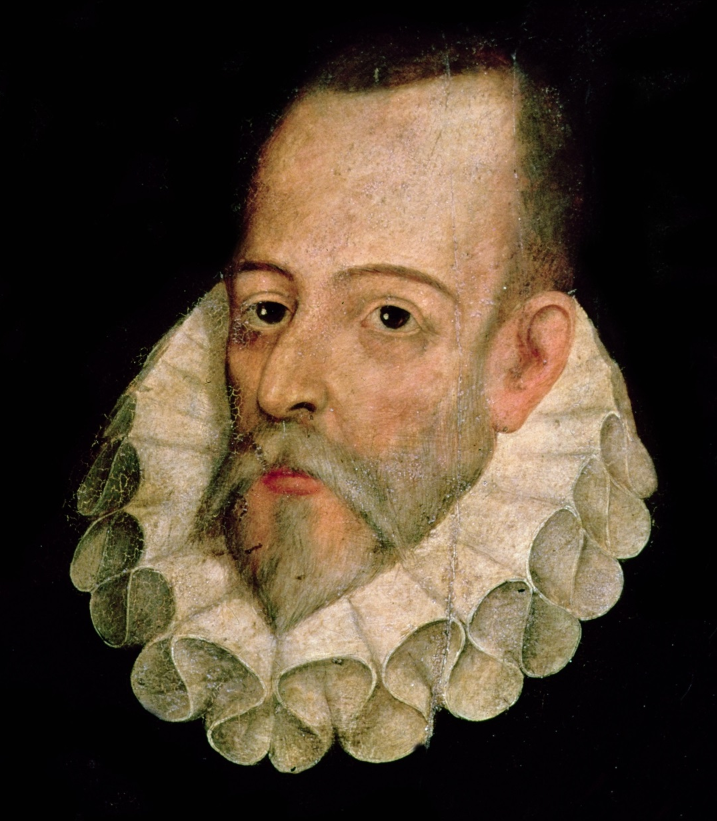
\includegraphics[width=0.55\linewidth]{figures/Servantes.png}
  \end{figure}
\end{minipage}

\graylink{wikipedia.org}
\end{frame}


\begin{frame}{Ближайшие соседи}

Зависимая переменная: $y_i$.

Предикторы: $x_i = (a_i, b_i, c_i, \ldots)$.
\pause

Расстояние между двумя наблюдениями:

\[
d(x_1, x_2) = \sqrt{(a_1 - a_2)^2 + (b_1 - b_2)^2 + (c_1 - c_2)^2 + \ldots}  
\]
\pause

\begin{block}{Естественное определение}
  \alert{Ближайшими соседями} наблюдения $x$ называем те наблюдения, расстояние от него до которых наименьшее. 
\end{block}

\end{frame}

\begin{frame}{Прогнозирование}

\alert{Цель}: построить прогноз для $x = (a, b, c, \ldots)$.

\pause

Выбираем $k = 3$ ближайших соседей данного наблюдения. 

\pause 

Допустим это оказались наблюдения номер $5$, $42$ и $100$.

\pause

Считаем прогноз для вектора предикторов $x$ как среднее:
\[
\hat y = \frac{y_5 + y_{42} + y_{100}}{3}.
\]
\end{frame}

\begin{frame}{Треугольники — соседи квадрата}

\begin{center}
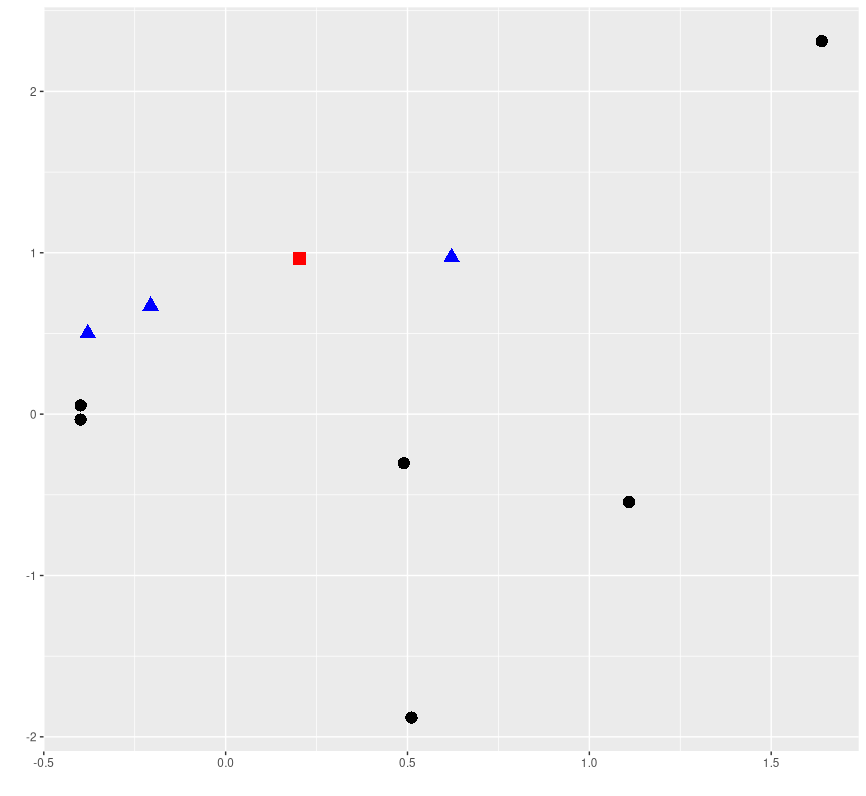
\includegraphics[scale=0.8]{figures/knn.png}
\end{center}

\end{frame}

\begin{frame}{Важность нормировки}

Расстояние \alert{чувствительно} к выбору масштаба.
\[
d(x_i, x_j) = \sqrt{(a_i - a_j)^2 + (b_i - b_j)^2 + (c_i - c_j)^2 + \ldots}  
\]

\pause

\alert{Важно} избавиться от единиц измерения!

\pause
Способ 1:
\[
a_i \to  \frac{a_i - \min(a)}{\max(a) - \min(a)}.
\]


\pause 

После преобразования все переменные лежат в отрезке $[0;1]$.

\pause

Данное масштабирование чувствительно к выбросам. 

\end{frame}


\begin{frame}{Избавиться от единиц измерения!}

  Способ 2:
  \[
  a_i \to \frac{a_i - \bar a}{\sqrt{\frac{\sum (a_j - \bar a)^2}{n - 1}}}.
  \]
  
  \pause 
  
  После преобразования каждая переменная имеет среднее равное нулю и 
  около 95\% её значений лежат в отрезке $[-2;2]$.
  
  \pause
  
  Данное масштабирование не учитывает выборочную корреляцию между переменными. 
  
\end{frame}



\begin{frame}{Избавиться от единиц измерения!}

  Способ 3: «метрика Махаланобиса»
  
  Матрицу центрированных переменных умножаем слева на корень из выборочной ковариационной матрицы.

\pause

Каждая новая переменная имеет среднее равное нулю и 
около $95\%$ её значений лежат в отрезке $[-2; 2]$.

\pause 
Новые переменные имеют нулевую выборочную корреляцию. 

\end{frame}


\begin{frame}{Как выбрать количество соседей?}

Основной способ: \alert{кросс-валидация}. 

\pause 
Для нескольких разных $k$, например, для $k \in \{1, 2, 3, 4, 5 \}$:

\begin{enumerate}[<+->]

\item Построим прогноз для каждого наблюдения, используя $k$ его ближайших соседей. 
\item Посчитаем сумму квадратов ошибок прогнозов
\[
  MSE_{k} = \frac{1}{n}\sum (y_i - \hat y_i^{cv})^2.
\]
\end{enumerate}
\pause
Выберем \alert{оптимальное} $k$.
\end{frame}



\begin{frame}{Задача классификации}


Что изменится, если $y$ — \alert{бинарная} переменная?  
\pause

Кратко: \alert{ничего}.

\pause
Зависимая переменная $y$ закодирована как $0$ и $1$, 
а $x_5$, $x_{42}$, $x_{100}$ — ближайшие наблюдения к $x$.


Считаем прогноз для вектора предикторов $x$ как среднее:
\[
\hat y = \frac{y_5 + y_{42} + y_{100}}{3}.
\]

\pause

Величина $\hat y$ — \alert{оценка вероятности} того, что $y = 1$.

\end{frame}

\begin{frame}{Метод $k$ ближайших соседей: итоги}

  \begin{itemize}[<+->]
    \item Предсказывает непрерывную или дискретную $y$.
    \item Не требует явного предположения \alert{о виде зависимости} от предикторов.
    \item Важно привести \alert{предикторы к общему масштабу}.
    \item \alert{Нет коэффициентов}, чтобы интерпретировать. 
    \item Можно комбинировать с другими методами.
  \end{itemize}
\end{frame}



% !TEX root = ../om_metrics_14.tex

\begin{frame} % название фрагмента

\videotitle{Мэтчинг}

\end{frame}



\begin{frame}{Мэтчинг: план}
  \begin{itemize}[<+->]
    \item Задача оценки эффекта влияния.
    \item Алгоритм мэтчинга.
    \item Мера склонности к воздействию. 
  \end{itemize}

\end{frame}


\begin{frame}{Цель анализа}

Данные:

$y_i \in \R$ — значение целевой переменной;

$a_i \in \{0, 1\}$ — индикатор того, что индивид $i$ получил воздействие;

$x_i \in \R$ — прочие характеристики индивида.

\pause

Хотим оценить \alert{влияние} бинарной переменной $a_i$ на $y_i$.

\end{frame}

\begin{frame}{Формализуем понятие «влияет»}

\alert{Гипотетические} значения:

$y_i(0)$ — значение целевой переменной, \alert{если бы} индивид не получил воздействие;

$y_i(1)$ — значение целевой переменной, \alert{если бы} индивид получил воздействие;

\pause 


\begin{block}{Задача}

Хотим оценить \alert{средний эффект воздействия}:

\[
ATE  = E(y_i(1) - y_i(0)).
\]
\end{block}


\end{frame}



\begin{frame}{А в чём проблема?}

\begin{block}{Задача}

    Хотим оценить \alert{средний эффект воздействия}:
    
    \[
    ATE  = E(y_i(1) - y_i(0)).
    \]
\end{block}

\pause

Наблюдаем \alert{только одну} из гипотетических величин!

У тех, кто получил воздействие, видим $y_i(1)$.

У тех, кто не получил воздействие, видим $y_i(0)$.

\[
y_i = y_i(a_i).  
\]


\end{frame}



\begin{frame}{Рандомизированный эксперимент}


\begin{block}{Рандомизированный эксперимент}
Воздействие $a_i$ назначается или выбирается случайно и не зависит от $y_i(0)$ и $y_i(1)$.

\[
  a_i \perp y_i(0), y_i(1)
\]

\end{block}

\pause
При назначении воздействия мы \alert{не предпочитаем} тех, кто на на него лучше среагирует. 


\alert{Нет самостоятельного выбора} воздействия индивидами, умеющими прогнозировать $y_i(0)$ и $y_i(1)$.

\end{frame}



\begin{frame}
  \frametitle{В мире розовых пони\ldots}

  В прекрасном мире \alert{рандомизированного эксперимента}:

  \alert{Любая} регрессия даст несмещённую и состоятельную оценку $ATE$.
  \pause
  \[
  \hat y_i = \hat \beta_1 + \hat \beta_a a_i,  
  \]
  \pause
  \[
  \hat y_i = \hat \beta_1 + \hat \beta_a a_i + \hat \beta_x x_i,  
  \]
  \pause
  В рандомизированном эксперименте:
  \[
  \plim_{n\to\infty} \hat \beta_a = ATE, \quad \E(\hat\beta_a) = ATE.  
  \]


\end{frame}

\begin{frame}{Отсутствие рандомизации}

  $y_i$ — результат теста по теории вероятностей;

  $a_i \in \{0, 1\}$ — пользовался ли студент шпаргалкой;

  $x_i$ — уровень знаний студента. 
  
  \pause
  Предположим, что только слабые студенты пользуются шпаргалкой. 
  \pause
  \[
    \hat y_i = \hat \beta_1 + \hat \beta_a a_i
  \]
  Регрессия недооценивает эффект, $E(\hat \beta_a) < ATE$.
\end{frame}


\begin{frame}{Отсутствие рандомизации}

  $y_i$ — результат теста по теории вероятностей;

  $a_i \in \{0, 1\}$ — пользовался ли студент продвинутым учебником;

  $x_i$ — уровень знаний студента. 
  
  \pause
  Предположим, что только сильные студенты пользуются продвинутым учебником. 
  \pause
  \[
    \hat y_i = \hat \beta_1 + \hat \beta_a a_i
  \]
  Регрессия переоценивает эффект, $E(\hat \beta_a) > ATE$.
\end{frame}



\begin{frame}
  \frametitle{Суровая реальность\ldots}

  Узнав о возможности получить воздействие, \alert{индивиды сами решают}, получать ли воздействие. 
  
  
  Значение $a_i$ \alert{связано с} $y_i(0)$ и $y_i(1)$. 

  \pause 

  В общем случае всё пропало, найти состоятельные и несмещённые оценки $ATE$ невозможно. 

  \pause 

  \begin{block}{Последняя надежда!}
  Воздействие не зависит от гипотетических исходов при фиксированном $x_i$.
  \[
  a_i \perp y_i(0), y_i(1) \mid  x_i
  \]
  \end{block}

\end{frame}


\begin{frame}{Мэтчинг и регрессия}

  \begin{enumerate}[<+->]
    \item Создаём кластеры исходных наблюдений. 
    
    В один кластер входят наблюдения с \alert{близкими} характеристиками $x_i$
    и разными значениями $a_i$.

    Внутри кластера $a_i$ не зависит от потенциальных исходов $y_i(0)$ и $y_i(1)$.

    \item Строим регрессию $y_i$ на $a_i$ с использованием \alert{весов} наблюдений 
    и с \alert{робастными стандартными ошибками}.

    Веса нивелируют различие в $x_i$ для получивших и не получивших воздействие. 

    Робастные стандартные ошибки учтут гетероскедастичность и 
    корреляцию внутри кластера. 
  \end{enumerate}




\end{frame}


\begin{frame}{Создаём кластеры наблюдений!}

  Кластеры бывают двух типов:
  \begin{itemize}[<+->]
    \item Один индивид, получивший воздействие, и несколько \alert{близких к нему} индвидов, не получивших воздействия. 
    \item Один индивид, не получивший воздействия, и несколько \alert{близких к нему} индвидов, получивших воздействие. 
  \end{itemize}

  При создании кластеров наблюдения получат веса.

  \pause
  Как выбрать близких индивидов к данному?
  \begin{itemize}[<+->]
    \item \alert{Расстояние Махаланобиса} для прочих характеристик $x_i$.
    \item \alert{Мера склонности} к воздействию (propensity score), $\widehat{ps}(x_i)$.
  \end{itemize}

\end{frame}

\begin{frame}{Мера склонности}

\begin{block}{Мера склонности}
Оценка вероятности получить воздействие, полученная с помощью прочих характеристик индивида $x_i$.
\[
\widehat{ps}(x_i) = \hat P(a_i = 1 \mid x_i).
\]
\end{block}
\pause
Например, можно оценить \alert{логистическую регрессию}
\[
  \hat P(a_i = 1 \mid x_i) = \Lambda(\hat\beta_1 + \hat\beta_x x_i),
\]
где $\Lambda(t) = \exp(t)/ (1 + \exp (t))$.

\end{frame}


\begin{frame}{Мера склонности и веса}
  \begin{block}{Мера склонности}
    Оценка вероятности получить воздействие, полученная с помощью прочих характеристик индивида $x_i$.
    \[
    \widehat{ps}(x_i) = \hat P(a_i = 1 \mid x_i).
    \]
  \end{block}
  \pause
  \begin{block}{Вес наблюдения}
    \[
      w_i = \begin{cases}
          1 / \widehat{ps}(x_i), \text{ если } a_i = 1; \\
          1 / (1 - \widehat{ps}(x_i)), \text{ если } a_i = 0; \\
      \end{cases}
    \]
  \end{block}
  \pause
  Вес наблюдения — насколько редко встречаются наблюдения с данным $a_i$ среди похожих по $x_i$. 
\end{frame}

\begin{frame}{Рецепт и большая наука}

\begin{block}{Краткий рецепт}
\begin{enumerate}
  \item Создаём кластеры наблюдений отличающихся только воздействием. 
  \item Оцениваем регрессию и получаем доверительный интервал для эффекта влияния.
\end{enumerate}
\end{block}

\alert{Важно:} наличие воздействия $a_i$ должно не зависеть 
от потенциальных исходов $y_i(1)$ и $y_i(0)$ при фиксированных $x_i$.

\pause

\begin{block}{Много интересного!}
  \begin{enumerate}
    \item ATE, ATT, ATM, непараметрические методы, \ldots
    \item Многие методы ещё не имеют глубокого теоретического обоснования. 
  \end{enumerate}
\end{block}
  
\end{frame}

\begin{frame}{Соседи и мэтчинг: итоги}

  \begin{block}{Общая идея}
    Метод ближайших соседей: используем похожие наблюдения, чтобы \alert{прогнозировать} $y_i$.
    
    Мэтчинг: используем похожие наблюдения, чтобы \alert{оценить эффект} $a_i$.
    \end{block}

\pause
    
  \begin{itemize}[<+->]
    \item Мэтчинг требует предположения $a_i \perp y_i(1), y_i(0) \mid x_i$.
    \item Мэтчинг — область активных исследований.
  \end{itemize}

\end{frame}

\end{document}





\end{document}
